%A description and illustration of the:

%Design and architecture of your ITU-MiniTwit systems

%All dependencies of your ITU-MiniTwit systems on all levels of abstraction and development stages. That is, list and briefly describe all technologies and tools you applied and depend on.

%Important interactions of subsystems.
    %For example, via an illustrative UML Sequence diagram that shows the flow of information through your system from user request in the browser, over all subsystems, hitting the database, and a response that is returned to the user.
    
    %Similarly, another illustrative sequence diagram that shows how requests from the simulator traverse your system.

%Describe the current state of your systems, for example using results of static analysis and quality assessments.

\section {System's Perspective}
\subsection{Design and Architecture}

\begin{figure}[H]
    \centering
    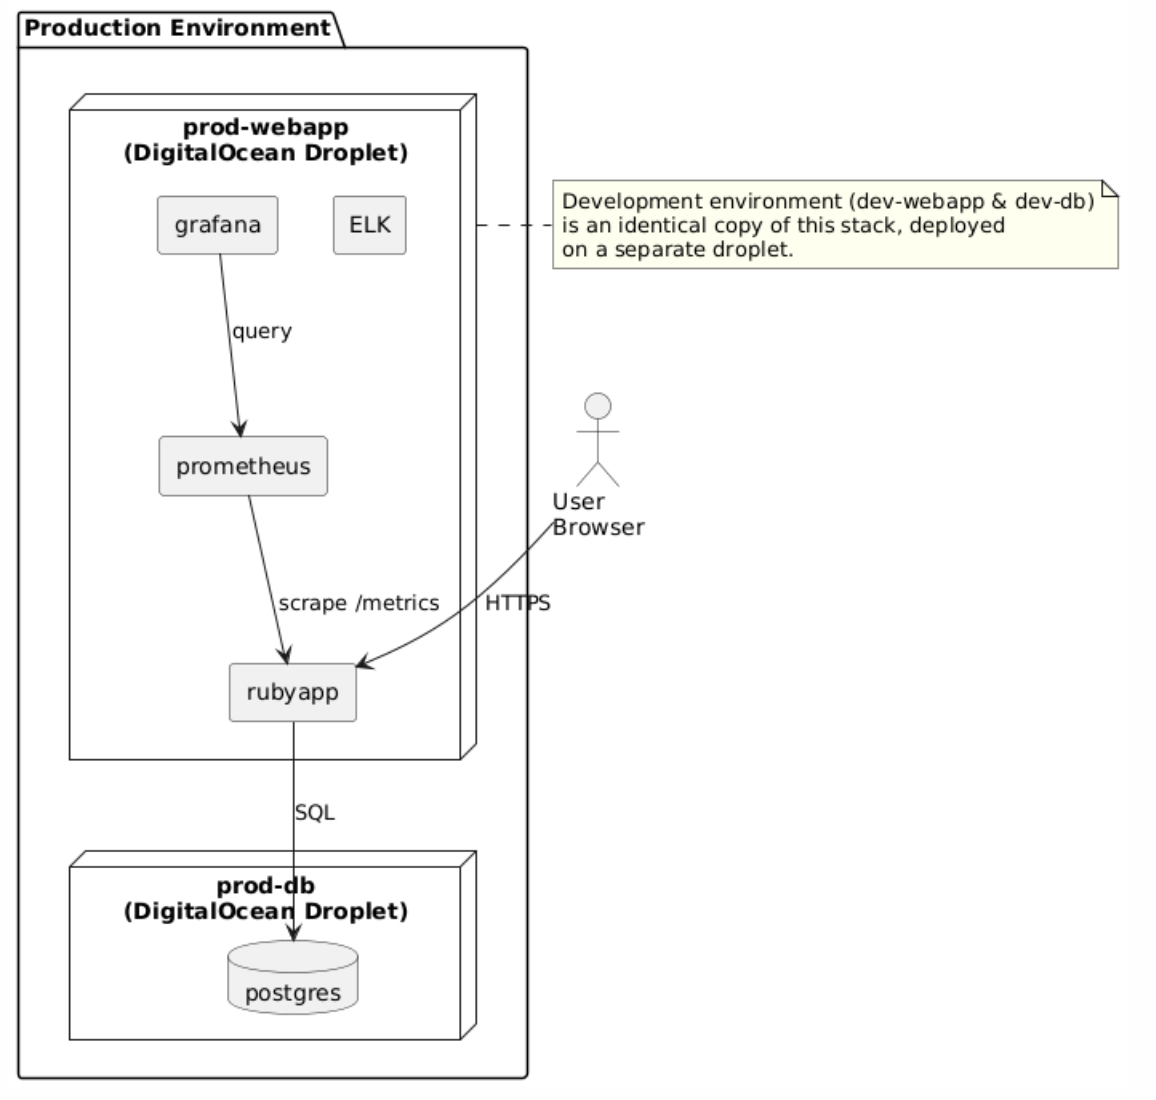
\includegraphics[width=1\linewidth]{images/deployment_diagram.png}
    \caption{Deployment Diagram}
    \label{fig:deployment}
\end{figure}

Figure~\ref{fig:deployment} presents the deployed architecture of \textit{MiniTwit} in production. The application uses 2 DigitalOcean droplets: 1 for application logic and 1 for a database. Splitting the droplets follows the principle of separation of concerns, as the webapp droplet is responsible for all logical tasks, as well as logging and monitoring, and the db droplet is only responsible for storage. Additionally this keeps our data safe, if the webapp droplet was harmed. \\

The application logic is build in Ruby and the database uses PostgreSQL as a database management system. We use ELK stack for logging, and Grafana with Prometheus for monitoring. \\

All these systems are containerized using docker. For example, postgres is not directly installed on the db droplet. Instead, a container is running of a docker image with support for postgres. The same goes for the webapp, logging and monitoring. The monitoring is 2 systems, grafana and prometheus, each running in their own containers. Grafana is for visualizing the data, and prometheus is a database, that keeps time-series data, that can then be queried to give insight into the activity. \\


\subsection{Dependencies}

Here follows a full list of all dependencies our systems rely on, with a short description of its purpose:

\subsubsection{Core Application Dependencies}
\begin{itemize}
    \item \textbf{sinatra} -- Web framework (similar to Flask in Python)
    \item \textbf{sequel} -- Database toolkit and ORM
    \item \textbf{sqlite3} -- SQLite database adapter
    \item \textbf{bcrypt} -- Password hashing
    \item \textbf{rack} \& \textbf{rack-test} -- Web server interface and testing
    \item \textbf{puma} -- Web server
    \item \textbf{pg} -- PostgreSQL adapter
    \item \textbf{rackup} -- Rack server launcher
    \item \textbf{rspec} -- Testing framework
    \item \textbf{rest-client} -- HTTP client library
\end{itemize}

\subsubsection{Database}
\begin{itemize}
    \item \textbf{Sequel gem} - ORM
    \item \textbf{PostgreSQL}
    \begin{itemize}
        \item Main production database, running off of a docker image
    \end{itemize}
    \item \textbf{SQLite3}
    \begin{itemize}
        \item Local database for testing, uses SQLite 3 module gem
    \end{itemize}
\end{itemize}

\subsubsection{Development \& Testing Dependencies}
\begin{itemize}
    \item \textbf{Testing Frameworks}
    \begin{itemize}
        \item \textbf{rspec} -- Ruby testing framework
        \item \textbf{dawnscanner} -- Security scanner
        \item \textbf{fasterer} -- Ruby performance analyzer
        \item \textbf{rubocop} -- Consistent code standards, style guide and formatting
    \end{itemize}
\end{itemize}

\subsubsection{CI/CD}
\begin{itemize}
    \item \textbf{Github Actions} used as the CI/CD platform for all workflows, and use the following templates:
    \begin{itemize}
        \item \textbf{actions/checkout@v4} -- Code checkout
        \item \textbf{ruby/setup-ruby@v1} -- Ruby environment setup
        \item \textbf{appleboy/ssh-action@v0.1.10} -- SSH deployment
        \item \textbf{softprops/action-gh-release@v1} -- GitHub release management
    \end{itemize}
\end{itemize}

\subsubsection{Development Environment}
\begin{itemize}
    \item \textbf{Vagrant Configuration}
    \begin{itemize}
        \item Digital Ocean provider
        \item Ubuntu 22.04 base image for both webapp and db
        \item Docker and Docker Compose installation
    \end{itemize}
\end{itemize}

\subsubsection{Security Dependencies}
\begin{itemize}
    \item \textbf{bcrypt} -- Password hashing
    \item \textbf{dawnscanner} -- Security scanning
\end{itemize}

\subsubsection{Monitoring \& Health Checks}
\begin{itemize}
    \item PostgreSQL health checks in Docker
    \item Database connection monitoring
    \item GitHub Actions for automated testing and deployment
\end{itemize} 

\subsection{Interactions of Sub-systems}

\begin{figure}[H]
    \centering
    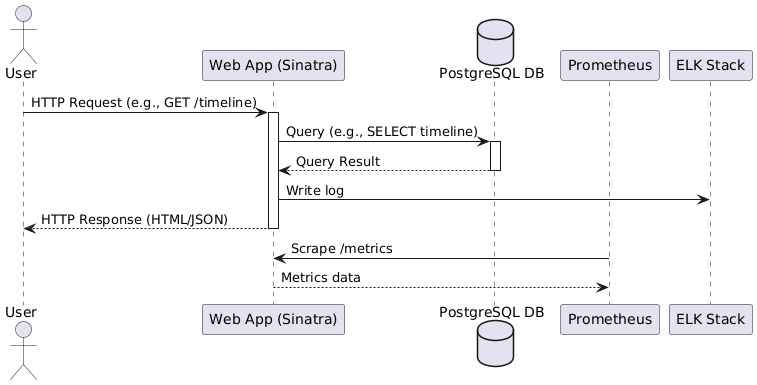
\includegraphics[width=1\linewidth]{images/sequence_user.png}
    \caption{sequence-user}
    \label{fig:seq-user}
\end{figure}

Figure~\ref{fig:seq-user} illustrates how a user-request flows through the deployed \textit{MiniTwit} system. When a user makes a request, for example accessing their timeline, the request is handled by the \texttt{webapp}, a Sinatra-based web application running as a container from a docker image. The application queries a PostgreSQL database for whatever data needed to fulfill the users request. \\

These request are directly relevant to serving the user's request, but also cause other effects. Sinatra sends data to out logging system and our monitoring system, to capture the activity it receives. The way it does logging, is similar to a print statement to standard output, but uses a specialized database, for handling these. For monitoring, we have an endpoint, '/metrics', dedicated to accumulating data, that Prometheus then captures and stores.\\

On top of this, we have api-endpoints, that allow automated systems to use the system without going through the UI. For example, the simulator will be using these endpoints. The flow of information after the requests, will be the same as for a user-request. 

\subsection{State of the system}

\begin{figure}[H]
    \centering
    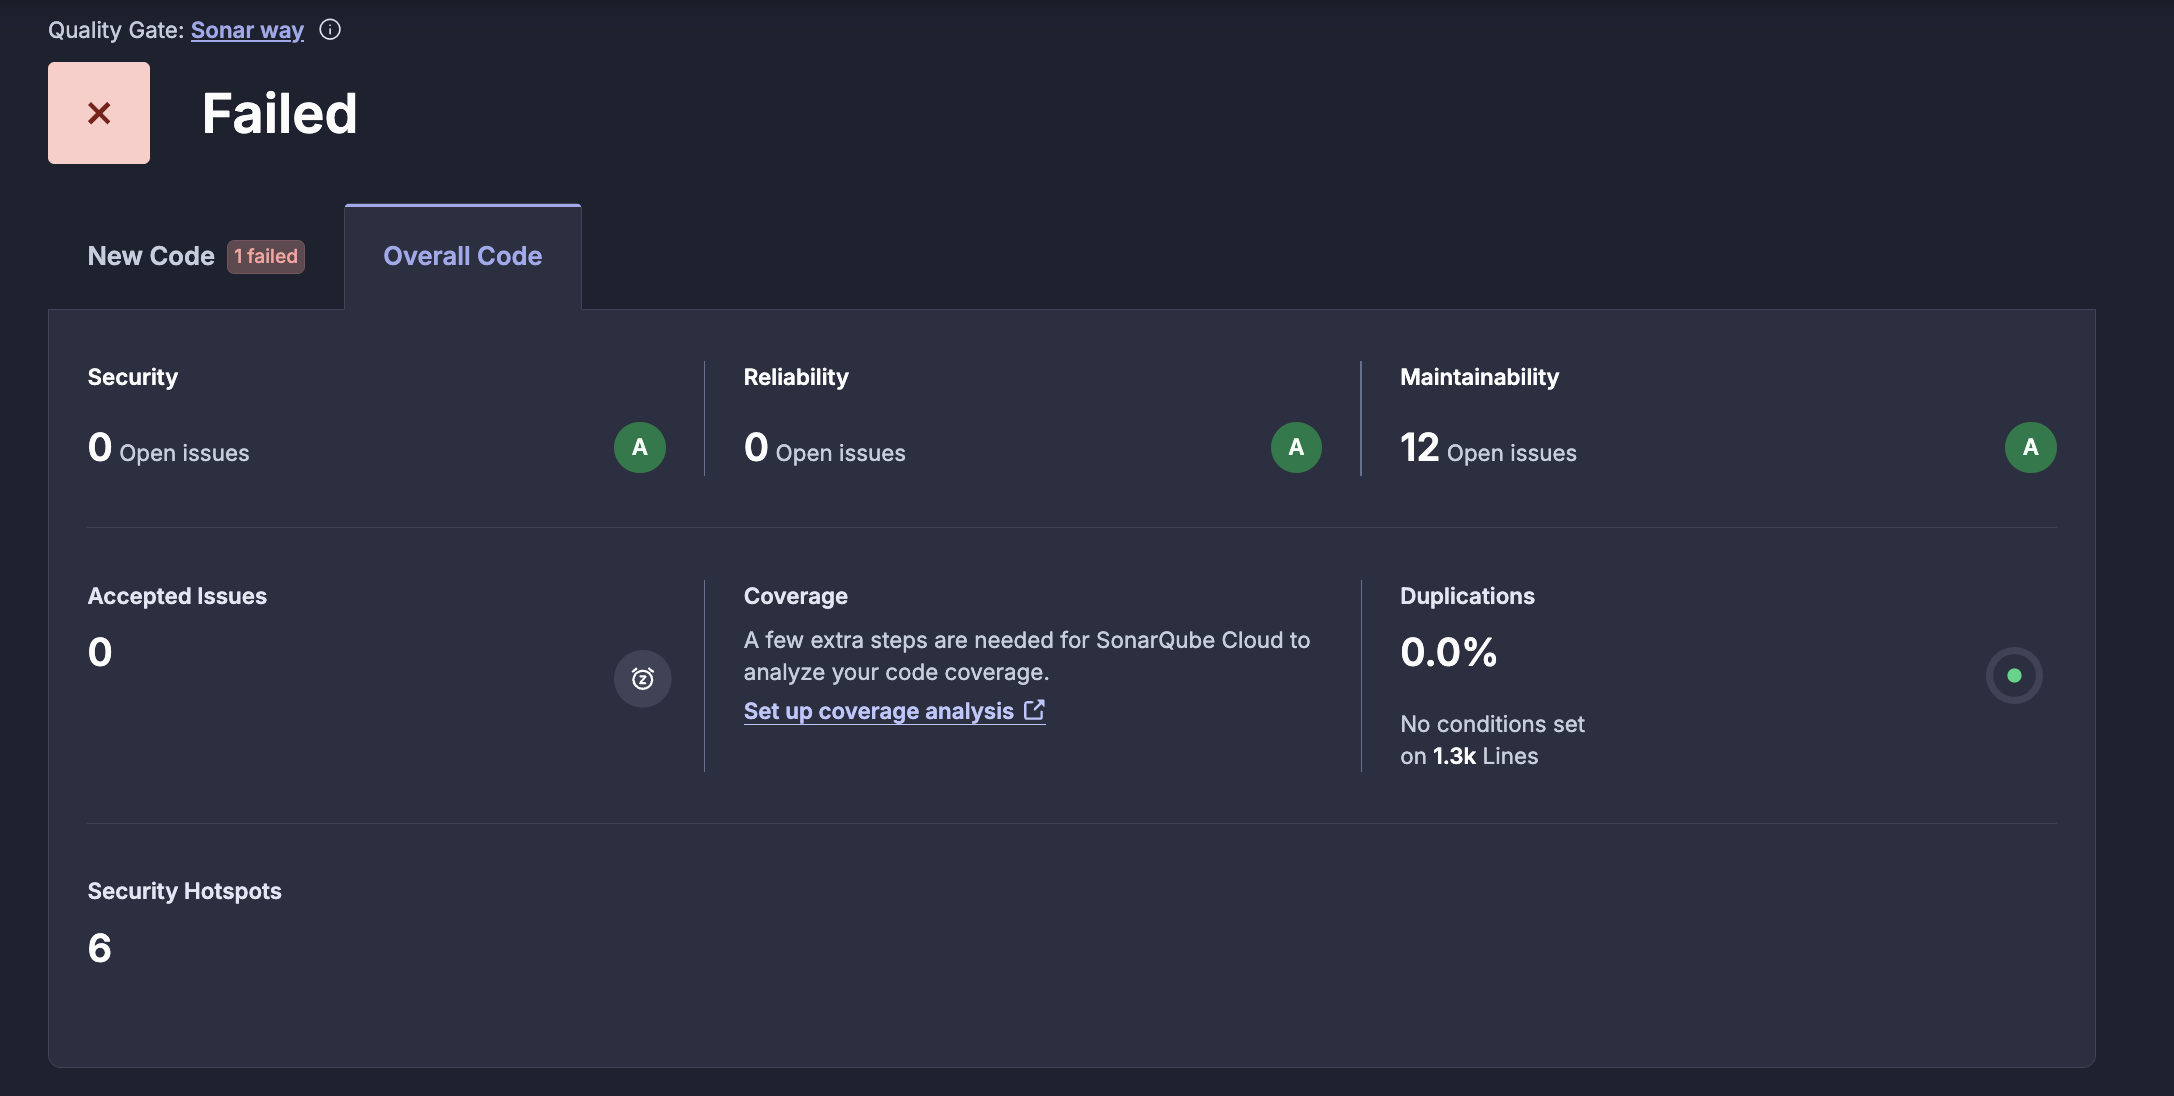
\includegraphics[width=1\linewidth]{images/sonarqube.png}
    \caption{SonarQube}
    \label{fig:sonarqube}
\end{figure}

We've used SonarQube for code analysis, in order to asses the quality of our code, for example in terms of maintainability, and to prevent human errors. As the figure \ref{fig:sonarqube} shows, we have a reasonably solid codebase, with some room for improvement. \\

First lets address the 6 Security Hotspot issues. 4 of these are related to the flag\_tool.cs file, which is not exposed to the internet anyway. The 2 others are about our docker containers running as root: \\

\begin{figure}[h]
  \centering
  \begin{minipage}[t]{0.45\linewidth}
    \centering
    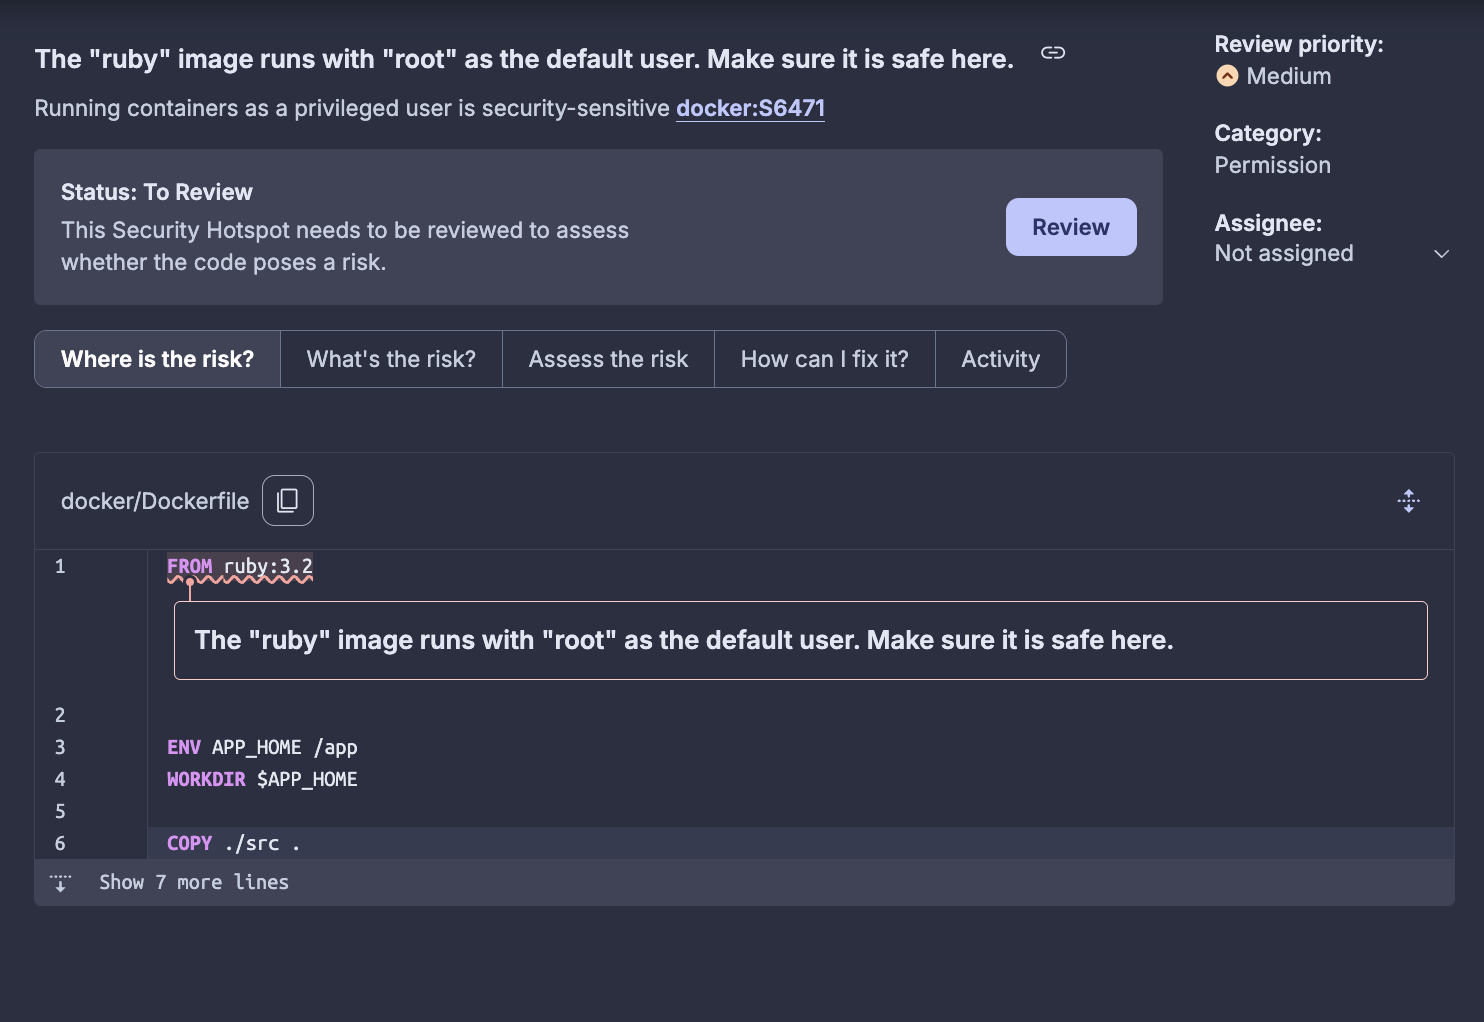
\includegraphics[width=0.9\linewidth]{images/sonarqube-ruby.png}
    \caption{Ruby container warning}
    \label{fig:ruby-warning}
  \end{minipage}%
  \hfill
  \begin{minipage}[t]{0.45\linewidth}
    \centering
    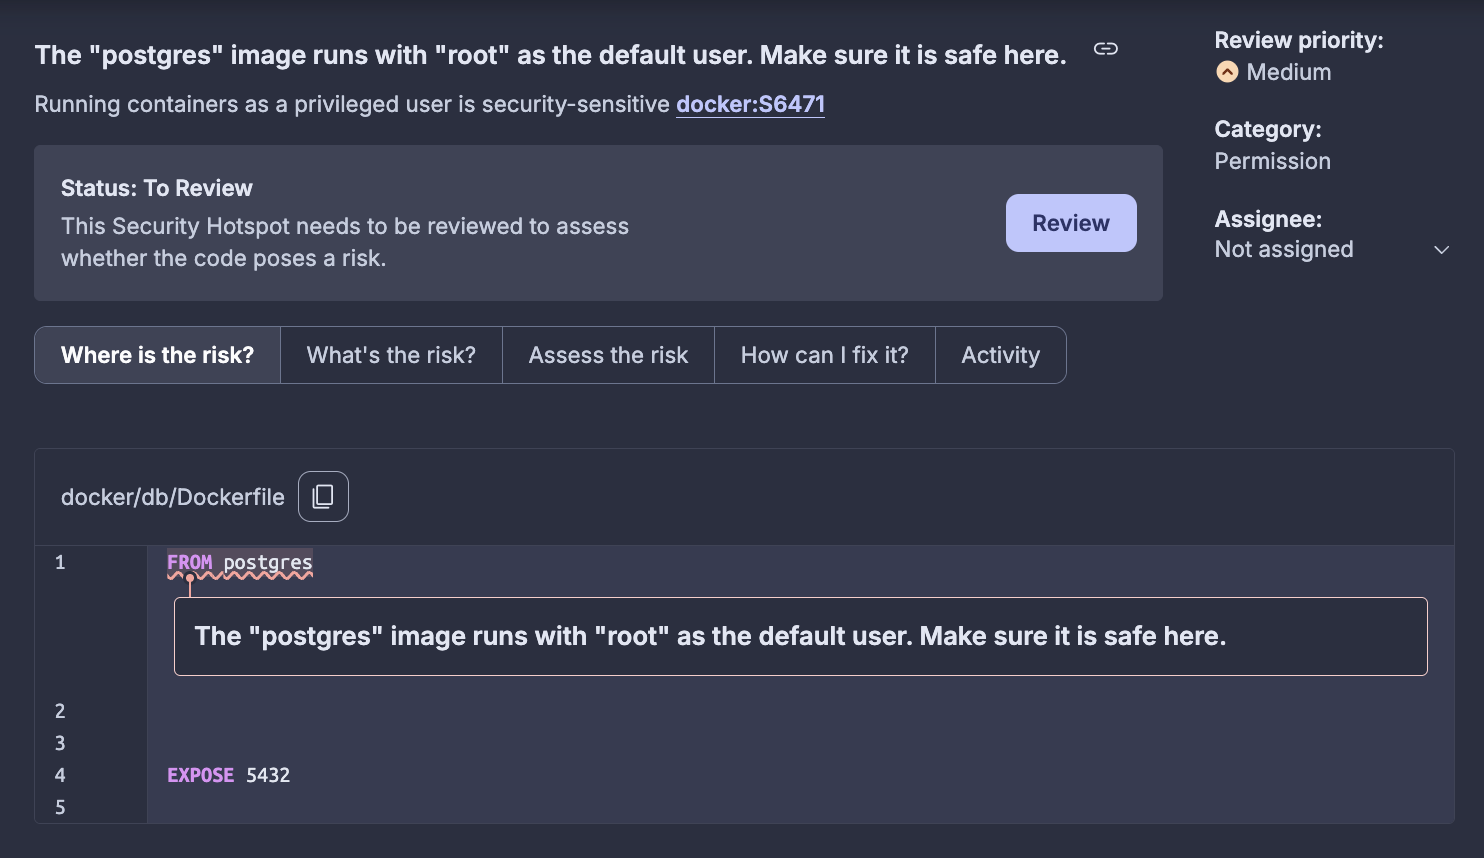
\includegraphics[width=0.9\linewidth]{images/warning_docker.png}
    \caption{PostgreSQL warning}
    \label{fig:postgres-warning}
  \end{minipage}
\end{figure}

Both warnings are about the default user being \texttt{root} inside the containers. We believe this to be a low-risk issue, because the containers run in isolated Docker environments without elevated host privileges or sensitive bind mounts. The web application interacts with the database exclusively through the Sequel ORM, and the PostgreSQL container is password-protected. While using a non-root user is a recommended hardening step, we determined that the current configuration does not introduce meaningful risk. \\

For maintainability issues, 8 of these are for flag\_tool.c, and 2 are for refactored\_minitwit\_tests.py, both files are not maintained, and thus not an issue. The last error is regarding a string literal used 3 times, which could be made into a variable. We believe this is manageable. \\

